\documentclass[journal]{IEEEtran}
\usepackage{amsmath,amssymb,graphicx,booktabs,array,url}
\usepackage{fontspec}
\setmainfont{Times New Roman}
\usepackage[hidelinks]{hyperref}
\usepackage{balance}
\newtheorem{proposition}{Proposition}
\newcommand{\R}{\mathbb{R}}
\newcommand{\norm}[1]{\left\lVert#1\right\rVert}
\newcommand{\um}{\,\mu\mathrm{rad}}
\def\ResultRows{
healthy & constant fit & 0/100 & NaN & 0.000 & 0.000 \\
healthy & projected fixed & 0/100 & NaN & 0.000 & 0.000 \\
healthy & DAP & 0/100 & NaN & 0.000 & 0.000 \\
pointing & constant fit & 100/100 & 0.13 & 2.689 & 2.800 \\
pointing & projected fixed & 100/100 & 0.12 & 2.689 & 2.800 \\
pointing & DAP & 100/100 & 0.16 & 2.740 & 2.800 \\
linear drift & constant fit & 0/100 & 0.99 & 11.760 & 2.800 \\
linear drift & projected fixed & 100/100 & 0.12 & 4.172 & 2.800 \\
linear drift & DAP & 100/100 & 0.16 & 4.265 & 2.800 \\
attenuation only & constant fit & 0/100 & 0.98 & 1.360 & 2.800 \\
attenuation only & projected fixed & 100/100 & 0.06 & 1.360 & 2.800 \\
attenuation only & DAP & 0/100 & NaN & 1.360 & 0.000 \\
quadratic drift & constant fit & 100/100 & 0.26 & 3.771 & 2.800 \\
quadratic drift & projected fixed & 100/100 & 0.12 & 3.771 & 2.800 \\
quadratic drift & DAP & 100/100 & 0.17 & 3.834 & 2.800 \\
fast fading & constant fit & 0/100 & 2.32 & 11.705 & 2.800 \\
fast fading & projected fixed & 0/100 & 1.55 & 11.705 & 2.800 \\
fast fading & DAP & 0/100 & 3.05 & 11.767 & 2.772 \\
deep loss & constant fit & 59/100 & 0.11 & 12.000 & 2.800 \\
deep loss & projected fixed & 59/100 & 0.11 & 12.000 & 2.800 \\
deep loss & DAP & 70/100 & 0.15 & 12.000 & 2.800 \\
near threshold & constant fit & 100/100 & 0.06 & 2.203 & 2.800 \\
near threshold & projected fixed & 100/100 & 0.06 & 2.203 & 2.800 \\
near threshold & DAP & 0/100 & NaN & 0.000 & 0.000 \\
dark & constant fit & 0/100 & NaN & 12.000 & 0.000 \\
dark & projected fixed & 0/100 & NaN & 12.000 & 0.000 \\
dark & DAP & 0/100 & NaN & 12.000 & 0.000 \\
}

\graphicspath{{results/full/}}
\begin{document}
\title{Drift-Projected Optical Fault Diagnosis With Service-Constrained Probe Selection}
\author{Research manuscript draft\\Author names and affiliations to be supplied}
\maketitle
\begin{abstract}
Received-power measurements cannot passively distinguish optical pointing error from scalar attenuation. Active angular excitation can resolve this ambiguity, but attenuation changing during the excitation biases a constant-gain fit, and the excitation itself can interrupt a working link. This paper develops a drift-projected diagnosis and finite-library probe-selection method for a two-axis optical terminal. The logarithmic Gaussian-beam model is projected orthogonally to a temporal nuisance subspace, producing an explicit identifiability condition, a conditional confidence bound, and an approximation-error bound. An eight-dwell sequence cancels affine temporal drift and attains the minimum-eigenvalue information bound for a specified quasi-static angular-energy budget. A trajectory-based selector trades information against excitation energy and a conservative outage surrogate; infeasible diagnosis is an explicit outcome. A reproducible benchmark integrates an existing nonlinear terminal model in MATLAB and evaluates nine scenarios, six methods, and 100 paired seeds, totaling 5,400 trials. With affine log-attenuation drift, mean outage falls from 11.7604~s for a constant-gain comparator to 4.2652~s, while projected fixed excitation achieves 4.1716~s. On near-threshold links, refusal to excite avoids the comparator's 2.2028~s of probe-induced outage, at the cost of obtaining no diagnosis. Fast fading defeats all tested estimators, and insufficient aligned power cannot be repaired by pointing. The evidence supports a focused simulation result rather than hardware reliability, constellation performance, or universal superiority.
\end{abstract}
\begin{IEEEkeywords}
Optical terminals, active fault diagnosis, identifiability, nuisance rejection, pointing recovery, experiment design.
\end{IEEEkeywords}

\section{Introduction}
An optical terminal can lose received power because its beam is misaligned or because its effective optical gain has decreased. These causes demand different responses. A pointing correction can compensate a boresight error; it cannot restore power that remains below receiver sensitivity even at perfect alignment. Acting on the wrong explanation consumes time and can interrupt an otherwise usable link. The distinction is particularly consequential when diagnostic information is obtained by deliberately moving the terminal.

Power-based optical tracking is established. Guelman \emph{et al.} developed cooperative extremum-seeking pointing for an intersatellite optical link \cite{guelman}. Fine-pointing actuators and their practical limitations are reviewed in \cite{milasevicius}. More generally, active diagnosis selects inputs that distinguish competing explanations of observed behavior. Input constraints and discrimination criteria have been studied by Cheong and Manchester \cite{cheong}. Palmer and Bollas explicitly address fault information in the presence of uncertainty \cite{palmer}. These works preclude treating dithering, information-driven input design, or nuisance rejection as new concepts.

The present study addresses a narrower interaction. A constant-gain optical regression uses samples collected at different times as if the gain were unchanged. A slow temporal gain change can therefore project onto the angular regressors. Meanwhile, a probe that improves identifiability can cross the receiver threshold. An estimator that ignores the first issue can reject an otherwise identifiable fault, whereas an input design that ignores the second can create the outage it was intended to prevent.

The proposed drift-annihilating probing method, abbreviated DAP, is a derivation for this measurement model rather than a collection of learning architectures. Its technical content is: (i) a nuisance-projected optical regression with a necessary and sufficient rank condition under stated assumptions; (ii) a balanced eight-dwell construction and an angular-energy information bound in the quasi-static limit; and (iii) a finite-library selector evaluated on predicted actuator motion, with explicit refusal when its information and service constraints cannot both be met. Projection and optimal experiment design are established tools. The potentially publishable contribution is their precise optical-terminal specialization and demonstrated information--service tradeoff; an exhaustive novelty claim is not made.

All quantitative evidence in this manuscript comes from the accompanying executed benchmark. Historical multi-satellite results in the source project are background and are not pooled with the new trials. The new experiment is a single-terminal evaluation. It does not establish orbital-network recovery or validate a complete flight fault-management system.

\section{Terminal Model and Diagnosis Problem}
\subsection{Mechanical and optical dynamics}
For two pointing axes, let $q\in\R^2$ denote terminal angle, $v\in\R^2$ angular rate, and $a\in\R^2$ delivered torque. The original project's mechanical equations are retained:
\begin{align}
 \dot q&=v,& J\dot v&=a-dv,\\
 \tau\dot a&=\eta_a u_c-a, &
 \norm{u_c}_\infty&\leq u_{\max}.
\end{align}
The implementation limits angular rate and includes the source model's anti-windup behavior. Here $\eta_a=1$ and the actuator lag is nominal in the primary experiment; actuator faults are not a target of the new optical estimator. Every method uses the existing PID controller option. The new simulations call the same \texttt{terminal\_kernel} implementation for the continuous derivatives and measurements from the local source project \cite{sourceproject}.

The source optical model is
\begin{equation}
 p(t)=p_0g(t)\exp\!\left[-\frac{2\norm{q(t)+b}^2}{\alpha^2}\right],
 \label{eq:power}
\end{equation}
where $b$ is a constant two-axis boresight offset during a diagnostic window, $g(t)>0$ is effective scalar gain, and $\alpha$ is divergence. With range $L$ and aperture radius $r_a$,
\begin{equation}
 p_0=P_t\eta_o\left[1-\exp\!\left(-\frac{2r_a^2}{L^2\alpha^2}\right)\right].
\end{equation}
Service availability is $\mathbf{1}\{p\geq p_{\min}\}$. The nominal values give $p_0\simeq3.9062~\mu\mathrm{W}$ and $p_{\min}=1.5~\mu\mathrm{W}$. The corresponding fault-free angular service radius is approximately $13.84\um$.

\begin{table}[t]
\caption{Retained physical parameters and new diagnostic settings}
\centering\footnotesize
\begin{tabular}{@{}p{0.30\columnwidth}p{0.34\columnwidth}p{0.26\columnwidth}@{}}\toprule
Parameter & Value & Role\\\midrule
Range $L$ & 800 km & Fixed geometry\\
Divergence $\alpha$ & $20\um$ & Gaussian angular scale\\
Transmit power $P_t$ & 0.5 W & Fixed, not boosted\\
Optical efficiency $\eta_o$ & 0.4 & Nominal\\
Aperture diameter & 0.10 m & Receiver\\
$J$, $d$, $\tau$ & 0.002, 0.004, 0.08 & Source dynamics, SI\\
$u_{\max}$, rate limit & $2~\mu$N m, $120\um$/s & Source limits\\
Sample time, duration & 0.02 s, 14 s & RK4 integration\\
Angle noise scale & $0.08\um$ & Source sensor model\\
Relative power noise & 0.008 & Source sensor model\\
Log-noise design floor & 0.03 & Conservative fitting floor\\
Target confidence radius & $1\um$ & Acceptance threshold\\
Offset prior radius $B$ & $30\um$ & Planner assumption\\
Log-gain slope bound $\ell$ & 0.15 s$^{-1}$ & Planner assumption\\
Service/acquisition budgets & 0 s / 4 s & Probe feasibility\\\bottomrule
\end{tabular}
\label{tab:params}
\end{table}

\subsection{Available measurements and nuisance model}
Only measured terminal angle, received power, and public nominal parameters enter the optical fit. Injection labels, fault onset, true offset, and future gain are excluded. The evaluator alone uses the injected quantities to calculate errors. Independent rate and torque measurements exist in the source project but are not used by the proposed optical regression.

Over one diagnostic window, write
\begin{equation}
 \log g(t_i)=\sum_{j=0}^{r}\gamma_j s_i^j+\rho_i,
 \qquad s_i=\frac{t_i-t_N}{t_N-t_1}.
\end{equation}
The default degree is $r=1$, giving exact rejection of affine log-gain drift. The remainder $\rho$ captures curvature, fast changes, and other mismatch. Changing effective gain is an abstract laser/channel-calibration disturbance here. Atmospheric scintillation is not assumed for a vacuum intersatellite path, and the chosen gain trajectories have not been calibrated against flight telemetry.

At a single fixed angle, infinitely many $(b,g)$ pairs produce the same $p$. No classifier can remove this structural ambiguity without additional assumptions or informative excitation. Darkness is more severe: when the detector provides no useful power, the logarithmic model is unavailable. The method returns uncertainty rather than labeling darkness uniquely as blockage, transmitter failure, or deep attenuation.

\section{Drift-Projected Estimation}
\subsection{Linearization by exact algebra}
Define $Q_i=q_i^T/\alpha$, $h=-4b/\alpha$, and
\begin{equation}
 z_i=\log(p_i/p_0)+2\norm{q_i}^2/\alpha^2.
\end{equation}
Expanding \eqref{eq:power} yields the exact regression
\begin{equation}
 z=V\beta+Qh+\rho+\epsilon,
 \label{eq:regression}
\end{equation}
where $V_{ij}=s_i^{j-1}$ and the constant entry of $\beta$ absorbs $-2\norm b^2/\alpha^2$. The additive $\epsilon$ model describes log-power noise in the theoretical analysis. The physical benchmark retains the source multiplicative power-noise model and angle noise, so the statistical assumptions are tested empirically rather than asserted to hold exactly.

Let $P_V=I-V(V^TV)^{-1}V^T$. In implementation a thin QR factorization computes $P_VQ$ and $P_Vz$ without forming a dense projector. Define
\begin{equation}
 F=Q^TP_VQ,\qquad
 \widehat h=F^{-1}Q^TP_Vz,\qquad
 \widehat b=-\alpha\widehat h/4.
 \label{eq:estimate}
\end{equation}
After estimating $h$, solve $V\widehat\beta=z-Q\widehat h$ in least squares. Since $s_N=0$, the end-of-window gain estimate is
\begin{equation}
 \widehat g_N=\exp(\widehat\beta_0+2\norm{\widehat b}^2/\alpha^2).
\end{equation}
This is an estimate at the last retained sample; it is not a forecast of future attenuation.

\begin{proposition}[Conditional identifiability]
Assume known $\alpha$, positive uncensored power, exact angles, a constant $b$, and $\rho=\epsilon=0$. If $V$ has full column rank, $b$ is uniquely identifiable jointly with the temporal nuisance coefficients if and only if $F\succ0$.
\end{proposition}
\emph{Proof:} Projection removes $V\beta$, leaving $P_Vz=P_VQh$. Its solution is unique exactly when $P_VQ$ has column rank two, equivalent to $F\succ0$. If the rank is deficient, a nonzero $d$ satisfies $P_VQd=0$, so $Qd$ lies in the column space of $V$ and can be absorbed into a different nuisance coefficient vector. The two offsets then produce identical observations. $\square$

Thus the number of samples alone is insufficient. Motion that is nearly a temporal trend can be highly informative for a constant-gain fit yet nearly uninformative after drift rejection. The rank must be checked after projecting the actual measured motion.

\subsection{Uncertainty and model mismatch}
Under exact angles, $\rho=0$, and independent Gaussian log noise with variance $\sigma^2$,
\begin{equation}
 \operatorname{Cov}(\widehat b)=\frac{\alpha^2\sigma^2}{16}F^{-1}.
\end{equation}
A ball containing the conventional 95\% two-dimensional confidence ellipse has radius
\begin{equation}
 R_{95}=\frac{\alpha\sigma}{4}
 \sqrt{\frac{\chi^2_{2,0.95}}{\lambda_{\min}(F)}}.
 \label{eq:radius}
\end{equation}
The code uses $\chi^2_{2,0.95}=5.991464547$ and a noise scale no smaller than the fixed 0.03 design floor. This ball is conservative under the stipulated model, not an unconditional flight confidence guarantee.

\begin{proposition}[Unmodeled-drift sensitivity]
In the noiseless-angle regression with deterministic remainder $\rho$, the bias attributable to that remainder satisfies
\begin{equation}
 \norm{\widehat b-b}\leq
 \frac{\alpha}{4\sqrt{\lambda_{\min}(F)}}\norm{P_V\rho}.
 \label{eq:bias}
\end{equation}
\end{proposition}
\emph{Proof:} Subtract the true parameters in \eqref{eq:estimate}. The error in $h$ is $(P_VQ)^+P_V\rho$. The operator norm of this pseudoinverse is $1/\sqrt{\lambda_{\min}(F)}$. Multiplication by $\alpha/4$ gives the result. $\square$

Equation~\eqref{eq:bias} does not make arbitrary drift harmless. Raising polynomial degree removes more temporal structure but also removes angular information and consumes degrees of freedom. The default affine model is therefore retained for the mismatched fast-fading experiment. Increasing model flexibility after observing evaluation outcomes would change the research question.

The fit is rejected if any retained power sample is below $0.005p_0$, if the information matrix is ill-conditioned, if $R_{95}>1\um$, or if log-regression RMS residual exceeds 0.06. The estimated offset must remain within $30\um$ and gain within $(0.01,1.6)$. These checks detect some model failures; a small residual alone does not prove model validity, since a nuisance component aligned with the angular regressors can remain hidden.

\section{Probe Construction and Service-Aware Selection}
\subsection{Balanced excitation and an information bound}
Consider eight equal-duration quasi-static dwells with dimensionless angular rows
\begin{equation}
 Q=\frac{a}{\alpha}
 \begin{bmatrix}
 1&0\\-1&0\\-1&0\\1&0\\0&1\\0&-1\\0&-1\\0&1
 \end{bmatrix}.
 \label{eq:balanced}
\end{equation}
For equally spaced sample times, both columns are orthogonal to a constant and to time. Consequently affine log-gain drift is removed without consuming the nominal angular information. With one sample per dwell, $F=4(a/\alpha)^2I_2$.

\begin{proposition}[Quasi-static energy bound]
For any two-axis design with total dimensionless angular energy $E=\norm Q_F^2$ and any orthogonal nuisance projector,
\begin{equation}
 \lambda_{\min}(Q^TP_VQ)\leq E/2.
\end{equation}
Equality holds when $P_VQ=Q$ and $Q^TQ=(E/2)I_2$. The sequence in \eqref{eq:balanced} attains equality for affine drift and equal dwell spacing.
\end{proposition}
\emph{Proof:} The smaller eigenvalue of a two-dimensional positive semidefinite matrix is at most half its trace. Orthogonal projection cannot increase squared Frobenius norm, so $\operatorname{tr}(Q^TP_VQ)=\norm{P_VQ}_F^2\leq E$. Equality requires isotropic information and no energy removed by projection. Direct summation verifies both temporal moments vanish for \eqref{eq:balanced}. $\square$

This result is a constrained specialization of familiar experiment-design principles; it is not a general optimality theorem for a moving actuator. During transients, commanded angles differ from measured angles. DAP therefore predicts each candidate using nominal terminal dynamics and evaluates the information matrix on the predicted settled motion. The estimator later repeats the calculation on measured angles. Only the latter determines whether the fit is accepted.

\subsection{Finite-library selection}
The candidate library contains amplitudes $a\in\{1,2,4,6\}\um$ and dwell times $d_p\in\{0.35,0.5\}$~s, all using \eqref{eq:balanced}. The last 40\% of each dwell is retained for the estimator. With the nominal dynamics, predicted radii for 0.35-s dwells are approximately 2.074, 1.037, 0.518, and $0.346\um$. Thus the 1-$\um$ requirement cannot be met merely by choosing the smallest amplitude.

For each candidate, assume the initial angle is zero, $\norm b\leq B$, exact current received power $p_c$, and $|\mathrm{d}\log g/\mathrm{d}t|\leq\ell$. At its predicted angle $q(t)$,
\begin{equation}
 \underline p(t)=p_c\exp\!\left[-\frac{4B\norm{q(t)}+2\norm{q(t)}^2}{\alpha^2}-\ell t\right]
 \label{eq:lower}
\end{equation}
is a lower bound under these assumptions. This follows by taking the ratio of \eqref{eq:power} at $q(t)$ and zero, applying $b^Tq\leq B\norm q$, and bounding gain reduction over time. The discrete predicted outage surrogate is
\begin{equation}
 C_p=\Delta t\sum_i\mathbf{1}\{\underline p(t_i)<p_{\min}\}.
\end{equation}
Candidates satisfy the information-radius constraint and $C_p\leq C_{\max}$. The budget is zero when the measured link is working and 4~s when it is already down. Among feasible candidates, the implemented score is
\begin{equation}
 J_p=T_p+0.03\,\Delta t\sum_i\norm{q_i/(1\um)}^2.
 \label{eq:score}
\end{equation}
The coefficient is a fixed numerical tradeoff used consistently across all evaluation seeds. If the feasible set is empty, DAP abstains. The search is exact over this eight-candidate library; no global optimum over all waveforms is claimed.

In the noisy dynamic benchmark, $p_c$ is measured and motion is predicted with a nominal model. Therefore $C_p$ is a conservative design surrogate, not a validated probabilistic or robust safety certificate. A certifiable implementation needs a power-measurement bound and an actuator tracking-error tube in \eqref{eq:lower}. This distinction is material: the present algorithm is service-aware but not flight-safety certified.

\subsection{Trigger and recovery decision}
Every active comparator uses the same causal residual trigger: a log-power deviation greater than 0.18 for three consecutive samples, after a 1-s warmup. Each method receives one diagnostic attempt, avoiding differences caused by repeated retries. Windows start when this trigger fires, not at a supplied fault time. Powers below the detector floor suppress probing for all methods.

A pointing correction $q_{\mathrm{ref}}=-\widehat b$ is applied only after an accepted fit with $\norm{\widehat b}>4\um$ and $p_0\widehat g_N>1.05p_{\min}$. The source reference limit is retained. The aligned-power check prevents futile steering when attenuation alone makes service impossible. There is no injected clearance event in the new benchmark and no clearance schedule is visible to the decision rule.

\section{Reproducible Evaluation}
\subsection{Comparators and scenarios}
The six methods are passive operation; a constant-gain fit with sequential fixed probes; an affine projected fit with the same sequential probes; an affine projected fit with balanced fixed probes; DAP without its service constraint; and complete DAP. All fixed probes use $6\um$ amplitude and eight 0.35-s dwells. The constant-fit comparator adapts the original V2 optical regression into the shared experimental wrapper. It is explicitly not the full V2 supervisor, whose detection, repeated verification, and other fault classes differ.

The two fixed projected comparators separate the estimator benefit from the sequence benefit. The unconstrained DAP ablation separates amplitude/energy selection from service refusal. Without these comparisons, an improvement could be incorrectly attributed to all elements of the proposed method.

The nine scenarios are: healthy operation; a constant pointing offset; that offset with affine log-gain decline; attenuation decline without an offset; pointing with quadratic log-gain decline; pointing with fast oscillating gain; pointing with deep scalar loss; attenuation to just above receiver sensitivity; and complete darkness. Faults persist from 2~s to the end, but the supervisor does not receive this time.

For seed $s$, the pointing magnitude is $(20+6\cos s)\um$ and its direction is $0.4+0.9\sin s$ radians. This gives a deterministic, reproducible distribution of magnitudes and directions rather than a single favorable fault. The affine gain is $\exp[-0.09(t-2)]$, the quadratic gain is $\exp[-0.008(t-2)^2]$, and the fast-fading gain is $\exp[-0.045(t-2)+0.16\sin(4(t-2))]$. Deep-loss gain is 0.18 and near-threshold gain is 0.41. These stress trajectories are specified experimental inputs, not measured spacecraft statistics.

Each scenario uses evaluation seeds 1001--1100. Every method receives the same time-indexed random sequence within a seed. A separate two-seed software-development check is excluded from the paper. That check initially used smaller offsets that generally did not interrupt service; the final 14--26-$\um$ range was selected before the full evaluation to exercise recovery near the source project's fault scale. This development choice is recorded in the protocol.

\subsection{Metrics, execution, and verification}
Outage is integrated over $[2,14)$~s. Reported offset errors are Euclidean errors of all computed finite estimates, including rejected fits; an error value is not evidence of an accepted diagnosis. Acceptance counts are always shown separately. Other metrics include angular excitation energy, probe duration, final two-second availability, false pointing corrections on zero-offset scenarios, and empirical coverage conditional on accepted fits. No diagnosis yields an undefined error rather than zero error.

MATLAB R2026a Update~3 executes fixed-step RK4 with a 20-ms step. The primary simulation loop completed in approximately 38~s on the execution host, excluding startup and figure generation; this is not an embedded real-time execution benchmark. Nine software checks cover temporal moments, the information equality, exact affine-drift invariance, rank rejection, darkness rejection, gain recovery, Gaussian-model coverage, service-feasibility rejection, and integrator convergence. A 400-draw Gaussian-model check produced 98.25\% ball coverage. Halving the integration step in the deterministic check changed final terminal angle by approximately $2.17\times10^{-13}$~rad. These checks do not replace validation against independent physical measurements.

For outage differences relative to constant fit, 2,000 paired bootstrap resamples provide descriptive 95\% intervals. Resampling is over seeds, and the same seed ordering is retained across methods. The intervals are not adjusted for multiple comparisons and should not be interpreted as an exhaustive hypothesis-testing campaign.

\begin{table*}[t]
\caption{Executed evaluation: 100 seeds per row. Error is the median over finite computed fits, including rejected fits. Acceptance is reported independently. NaN means no finite estimate. Full six-method records are supplied in the result files.}
\centering\small
\begin{tabular}{llrrrr}\toprule
Scenario & Method & Accepted & Error ($\mu$rad) & Mean outage (s) & Mean probe (s)\\\midrule
\ResultRows
\bottomrule\end{tabular}
\label{tab:results}
\end{table*}

\begin{figure*}[t]
\centering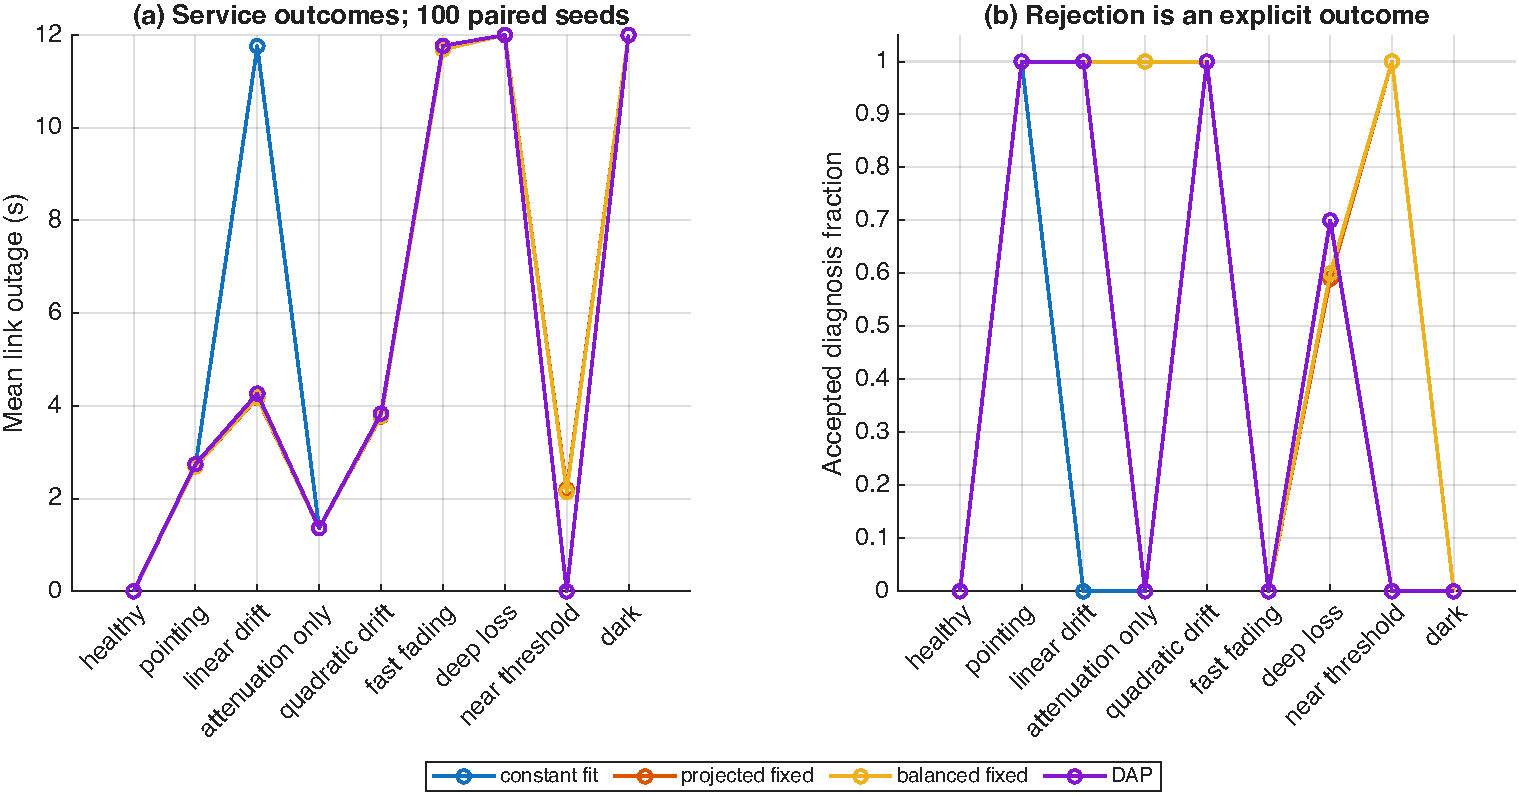
\includegraphics[width=\textwidth]{comparison.pdf}
\caption{Mean outage and diagnostic acceptance across all scenarios. The full proposed method trades diagnostic coverage for service preservation. Projected fixed excitation can recover slightly faster than the energy-selected probe. Healthy and dark scenarios have no accepted fit for different reasons: no anomaly trigger in the former, detector-floor rejection in the latter.}
\label{fig:comparison}
\end{figure*}

\begin{figure*}[t]
\centering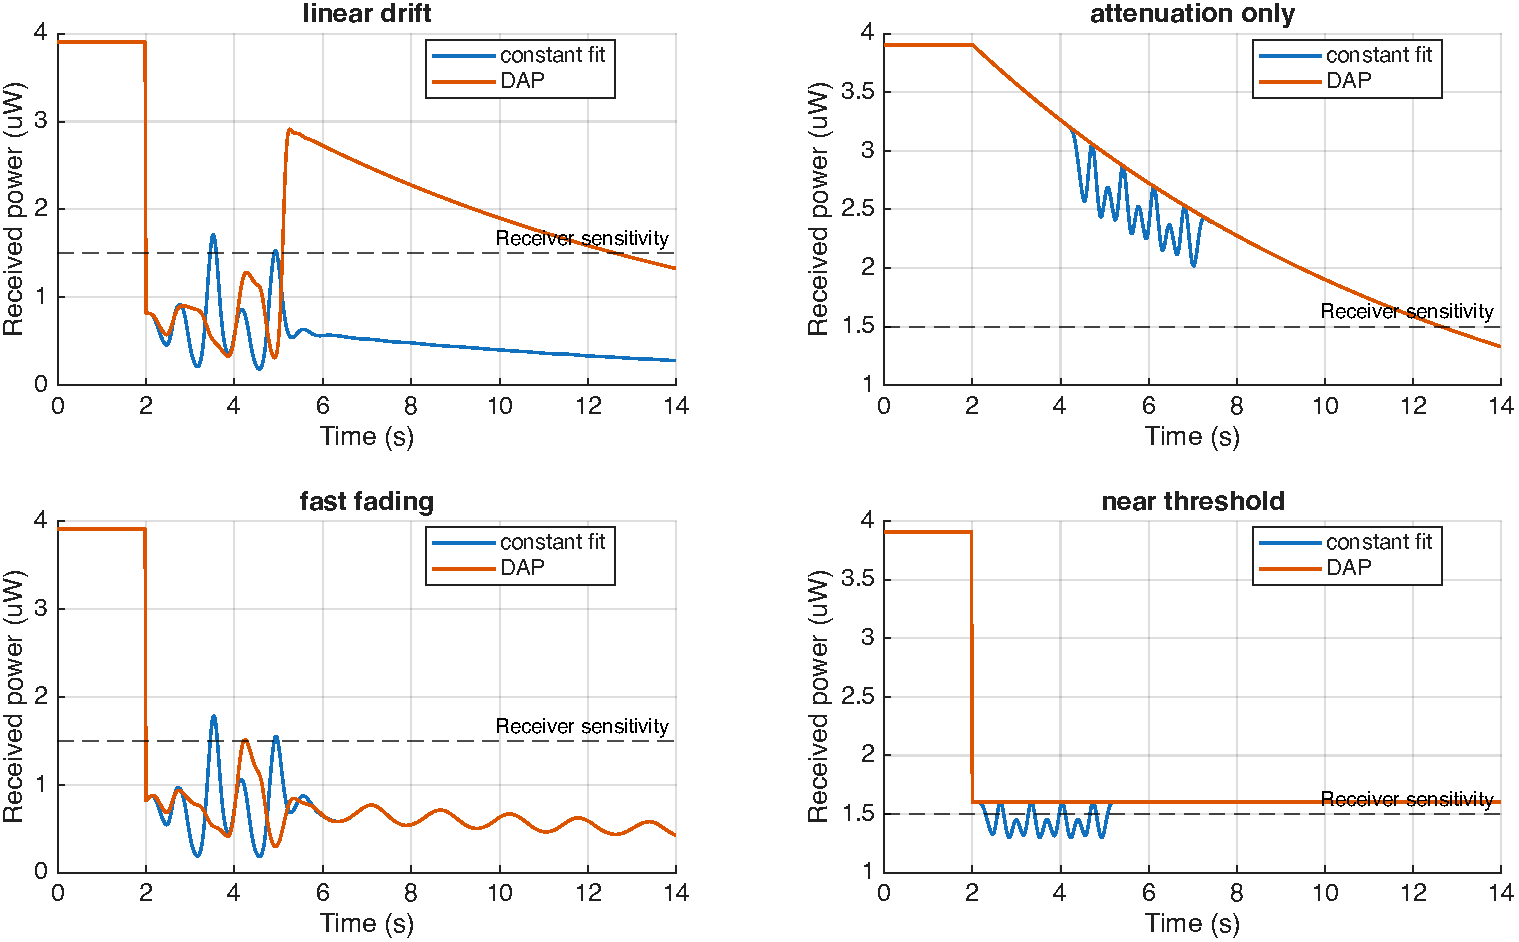
\includegraphics[width=0.98\textwidth]{traces.pdf}
\caption{Representative received-power traces for evaluation seed 1001. The selection of the first evaluation seed is fixed rather than chosen for visual advantage. Linear drift permits temporary pointing recovery; attenuation-only decline eventually exceeds the available optical budget; fast fading defeats the affine model; and near-threshold service is preserved by refusing excitation.}
\label{fig:traces}
\end{figure*}

\section{Results and Interpretation}
\subsection{Separation of affine drift from pointing}
Under affine log-gain decline, the constant-fit comparator produces median offset error $0.9925\um$, but all 100 fits fail the common residual/acceptance checks. Its mean outage is 11.7604~s. Projection with the identical sequential input reduces median error to $0.1243\um$, accepts all 100 fits, and reduces mean outage to 4.1716~s. This matched-input comparison is the strongest evidence for the estimator contribution; it does not rely on changing the probe or the trigger.

Complete DAP gives median error $0.1635\um$ and mean outage 4.2652~s, a 63.73\% reduction relative to constant fit. The paired outage difference is $-7.4952$~s with bootstrap interval approximately $[-7.5128,-7.4769]$~s. DAP's selected amplitude is $4\um$, and mean angular excitation energy is 28.5500~$\mu$rad$^2$~s, compared with 60.5991 for sequential fixed excitation and 64.2401 for balanced fixed excitation. The energy reduction relative to the sequential comparator is 52.89\%.

This is an energy--recovery tradeoff. The larger fixed projected probe has slightly smaller outage and lower error than complete DAP. Balanced fixed excitation gives the lowest median error among these linear-drift cases, $0.1085\um$, but does not have the shortest outage. The quasi-static information theorem therefore should not be presented as evidence that balanced probes dominate every dynamic performance measure.

The final two-second availability under affine attenuation is approximately 0.32 for all successful projected methods. Gain continues to decline after the pointing correction and eventually crosses the aligned-power threshold. A successful pointing correction does not create optical power. It is consequently inaccurate to describe these runs as uninterrupted or permanent link recovery.

\subsection{Steady gain and curvature mismatch}
With a constant pointing error and steady gain, constant fit is already effective: all 100 fits are accepted and mean outage is 2.6892~s. DAP also accepts all fits, but mean outage is 2.7404~s. The difference is $+0.0512$~s with interval approximately $[0.0248,0.0778]$~s. DAP consumes less angular energy but does not improve recovery speed in this condition.

For the specified quadratic decline, the constant fit has median error $0.2579\um$ and mean outage 3.7710~s. The sequential projected fit reduces error to $0.1244\um$ while changing mean outage only to 3.7708~s. DAP has error $0.1688\um$ and mean outage 3.8336~s. Mild curvature over the short window is small enough for the affine approximation to work in this test; no exact cancellation of quadratic drift is claimed. The quadratic gain slope also exceeds the planner's assumed slope bound late in the trial, so no all-trial service guarantee follows.

\subsection{Refusing harmful excitation}
In the near-threshold scenario, a perfectly aligned link with $g=0.41$ is usable. The fixed sequential probe creates 2.2028~s of outage on average. Removing the service constraint from DAP reduces this to 1.3186~s through its smaller amplitude, but still interrupts service. Complete DAP rejects the probe in all 100 trials and produces zero outage, matching passive operation. The paired difference from constant fit is $-2.2028$~s, with interval approximately $[-2.2042,-2.2014]$~s.

The price is complete diagnostic abstention: no boresight estimate or confirmed attenuation diagnosis is obtained. This is not a recovery success, since the link never needed recovery. Rather, it demonstrates that diagnostic excitation can be unnecessary and harmful. Attenuation-only decline produces a similar abstention tradeoff. DAP avoids probing but cannot prevent the subsequent power-limited outage of 1.36~s, which also occurs in passive operation.

Healthy trials produce no probes, no false pointing corrections, and no outage. None of the zero-offset evaluation cases causes an accepted pointing correction. This zero count is limited to the listed simulation conditions and is not a field false-alarm guarantee.

\subsection{Failures and irrecoverability}
All methods fail to produce an accepted fit under the specified fast-fading stress. DAP mean outage is 11.7666~s, compared with 11.7054~s for constant fit. The affine nuisance model is inadequate, and projection alone does not solve that mismatch. Reporting only the successful affine-drift case would conceal this important boundary.

With deep loss, perfectly aligned power is $0.18p_0\simeq0.7031~\mu$W, below sensitivity. Every method therefore has 12~s of outage. DAP accepts 70 of 100 diagnostic fits, versus 59 for the constant and sequential projected comparators, because smaller excitation leaves more measurements above the diagnostic floor. It correctly avoids a pointing correction that cannot restore service under the aligned-power check. Acceptance does not imply recoverability.

All active methods refuse to probe complete darkness and produce no diagnosis. Darkness is consistent with multiple physical causes; no uniquely identified blockage is reported. The real operational response would require alternative telemetry, an acquisition mode, or network-level redundancy, none of which is evaluated by this single-terminal experiment.

\subsection{Additional sensitivity experiments}
After the primary evaluation, a separately specified sensitivity protocol used 100 new paired seeds, 2001--2100. It compared constant fit, sequential projected fit, and DAP on pointing, affine drift, near-threshold gain, and fast fading under three conditions: fivefold angle and power noise; true inertia increased by 25\% and true actuator lag by 50\%, retaining the nominal planner library; and halved integration/sample step with a matching nominal library. These 3,600 additional trials are exploratory and are not pooled with the 5,400 primary trials.

Fivefold noise exposes a substantial weakness. Under affine drift, neither fixed comparator accepts a fit, while DAP accepts only one of 100; DAP outage rises to 11.7498~s. In the near-threshold case, noisy power sometimes makes the measured link appear down, enabling the acquisition budget: DAP accepts seven fits and has mean outage 0.0910~s, versus 2.2080~s for the fixed probes. Thus the zero-outage primary result does not persist unconditionally under increased measurement noise. An implementable robust service gate needs uncertainty on the current link state, not just an instantaneous power comparison.

With actuator mismatch, the sequential projected method and DAP still accept all affine-drift fits, with mean outages 4.1448 and 4.2990~s, respectively. DAP continues to refuse the near-threshold probe and produces zero outage there. This is evidence of tolerance to the specified mismatch only, not a general robustness guarantee. With a halved step, affine-drift outages are 4.1291~s for sequential projection and 4.3076~s for DAP, with all fits accepted. The change includes both numerical integration and measurement/control sampling, so it is not a pure integrator-convergence experiment. Fast fading remains unresolved in every sensitivity condition. Complete sensitivity metric rows and acceptance counts are supplied separately.

\subsection{Separate Simulink compatibility check}
A separately saved four-satellite Simulink model replaces only V2's optical-fit routine with the projected estimator. It retains V2's original probe and supervision logic and therefore does not implement the complete DAP planner. Original and adapted models were each executed for healthy and pointing scenarios at seed 101. Healthy service and diagnosis metrics match. For pointing, affected-link outage is 3.92~s with the adapter versus 3.82~s for original V2; exact isolation is 74.67\% versus 76.33\%. Both recover, but the additional nuisance parameter slightly delays inference in this steady-gain example. These four executions establish compatibility of the estimator interface, not network-level superiority or validation of the full new method.

\section{Limitations and Research Scope}
The mathematical results require a known Gaussian angular scale, a constant offset within a fit window, sufficiently accurate angle telemetry, and uncensored power. Encoder bias, unmodeled beam shape, receiver-side pointing, and uncertain divergence can violate these assumptions. A biased angle channel can be observationally confounded with boresight error. No result here establishes joint sensor/actuator/optical multifault isolation.

The service surrogate assumes a bounded offset, bounded log-gain slope, and a known nominal trajectory starting near zero. Actual measurement noise is unbounded in the simulated Gaussian model, and actuator prediction errors are not enclosed by a proved tube. Thus empirical preservation of service on the tested near-threshold links does not establish a robust safety guarantee. A formal safety claim requires additional analysis and independently measured parameter bounds.

The benchmark has one terminal, fixed range, a simplified receiver threshold, and one diagnostic attempt per trial. It excludes orbital motion, point-ahead geometry, acquisition uncertainty, routing, queues, moving ground stations, and hardware latency. The PID configuration differs from some historical sliding-mode runs in the source project. Existing network experiments cannot be appended to the new terminal results as though they validate the same new algorithm.

Comparators establish internal attribution but not superiority to the broader literature. In particular, a tuned lock-in/extremum-seeking tracker, a joint state/parameter filter, and a robust constrained active-diagnosis implementation should be reproduced under matched sensing and actuator budgets. The current constant-fit comparator often rejects rather than making an unsafe correction; its poor affine-drift recovery is evidence of a model limitation, not evidence that every existing optical tracker fails.

Before a Transactions submission, the main remaining evidence is an independent prior-art assessment of the exact optical specialization, stronger matched literature baselines, sensitivity to measurement/beam/actuator uncertainty, and a hardware-in-the-loop or optical-bench test. The finite-library score and the gain trajectories also require physical motivation. These are substantive research needs, not formatting tasks. IEEE Transactions on Aerospace and Electronic Systems has a direct spacecraft-system scope \cite{taesscope}; the two supplied application papers are structural writing references and do not establish the appropriate venue or the novelty threshold for this topic.

\balance
\section{Conclusion}
A log-Gaussian optical model admits exact removal of a specified temporal attenuation subspace before estimating a constant pointing offset. The resulting rank condition exposes when excitation is informative, and a balanced sequence attains an angular-energy information bound in the quasi-static setting. A finite-library selector can use that information condition while explicitly refusing probes that exceed its service surrogate.

Executed simulations support three bounded conclusions: affine-drift projection improves diagnosis relative to the matched constant-gain fit; smaller selected excitation reduces angular energy with a small recovery-delay penalty; and service-constrained refusal prevents probe-induced outage on the tested near-threshold links while sacrificing diagnosis. Fast fading, darkness, and insufficient aligned power remain unresolved. These results define a reproducible research candidate and its failure boundaries, rather than establish a universally superior or flight-validated recovery algorithm.

\section*{Reproducibility and AI Assistance}
Source, frozen protocol, all 5,400 trial metric rows, representative traces, aggregate tables, and MATLAB binary records accompany this draft in \texttt{research/v3}. The new code reuses the local project's original terminal model; attribution and licensing of that source must be resolved by the human authors before external distribution. The local Git remote differs from the repository URL supplied for this task, and no source ownership is inferred from either URL.

OpenAI Codex was used to develop the research formulation, draft all manuscript sections, implement the new experiment and analysis code, search for prior work, and generate figures and tables from executed MATLAB outputs. The manuscript, mathematical claims, source attribution, and reported evidence require human author verification before submission. This disclosure describes substantive assistance and follows IEEE's published disclosure guidance \cite{aipolicy}. No author names, affiliations, approvals, experimental hardware, or field data have been invented.

\begin{thebibliography}{9}
\bibitem{guelman} M. Guelman \emph{et al.}, ``Acquisition and pointing control for inter-satellite laser communications,'' \emph{IEEE Trans. Aerosp. Electron. Syst.}, vol. 40, no. 4, pp. 1239--1248, 2004, doi: 10.1109/TAES.2004.1386877.
\bibitem{milasevicius} M. Mila\v{s}evi\v{c}ius and L. Ma\v{c}iulis, ``A review of mechanical fine-pointing actuators for free-space optical communication,'' \emph{Aerospace}, vol. 11, no. 1, Art. no. 5, 2024, doi: 10.3390/aerospace11010005.
\bibitem{cheong} S. Cheong and I. R. Manchester, ``Input design for model discrimination and fault detection via convex relaxation,'' in \emph{Proc. American Control Conf.}, 2014, pp. 684--690, doi: 10.1109/ACC.2014.6859400. Author preprint: \url{https://arxiv.org/abs/1310.7262}.
\bibitem{palmer} K. A. Palmer and G. M. Bollas, ``Active fault diagnosis for uncertain systems using optimal test designs and detection through classification,'' \emph{ISA Trans.}, vol. 93, pp. 354--369, 2019, doi: 10.1016/j.isatra.2019.02.034.
\bibitem{taesscope} IEEE AESS, ``IEEE Transactions on Aerospace and Electronic Systems: scope.'' Accessed Oct. 23, 2026. \url{https://ieee-aess.org/publications/taes}.
\bibitem{aipolicy} IEEE CASS, ``Using AI-generated content in an IEEE article.'' Accessed Oct. 23, 2026. \url{https://ieee-cas.org/publications/using-ai-generated-content-ieee-article}.
\bibitem{sourceproject} ``Active fault diagnosis and verified recovery for multi-satellite optical communication,'' local source checkout, Git commit \texttt{0bc453ffa0ad}; original terminal implementation and V2 revision. Local configured remote: \href{https://github.com/Rishithachappidi/Active-Fault-Diagnosis-and-Verified-Recovery-for-Multi-Satellite-Optical-Communication}{source repository (GitHub)}.
\end{thebibliography}
\end{document}
